%************************************************
\chapter{Pruebas de Conocimiento Cero}\label{ch:zkp} 
%************************************************

% REF
% Fundamentals
% https://es.wikipedia.org/wiki/Prueba_de_conocimiento_cero
% https://en.wikipedia.org/wiki/Interactive_proof_system
% 


% Intro
% Ejemplo intuitivo del laberinto
% Pruebas interacticas: completitud y solvencia/solidez/robustez == completo y robusto/sólido, apartado corto, poner QR en el siguiente
% Prueba de conocimiento cero
%	Perfect vs Comp.
%	QR: es Perfect ZKP, y aplicaciones (id de Shamir, ...)
%	

% TODO: teorema de que el logaritmo discreto tiene un ZKP (para Schnorr). Buscar si existe demostración, por si no es perfect



Las pruebas de conocimiento cero, con siglas ZKP del inglés \textit{Zero-Knowledge Proofs}, permiten demostrar la veracidad de una declaración, sin revelar nada más de ella. En las ZKP intervienen dos partes, el \textit{Prover} y el \textit{Verifier}, o probador y verificador. El prover asegura que una declaración es cierta, y el verifier quiere convencerse de ello a través de una interacción con el prover, de modo que al final de la misma, o bien acaba convencido de que la declaración es cierta, o bien descubre, con una alta probabilidad, que el prover mentía.

Las pruebas de conocimiento cero surgen a partir de los sistemas de pruebas interactivas, que forman una parte importante de la teoría de complejidad computacional, y pidiendo la propiedad de \textit{conocimiento cero} obtenemos el subconjunto de sistemas interactivos que conforman las pruebas de conocimiento cero.

Las referencias para este capítulo se pueden encontrar en %TODO


\section{Una pequeña historia}
%Wikipedia

Antes de estudiar formalmente las ZKP, vamos a ver un ejemplo que se publicó originalmente como un cuento sobre la cueva de Alí Babá \citep{ZKPcave:story}, pero que aquí adaptamos para resumirlo.

\hfil

Imaginemos una cueva donde el camino se bifurca y al final de cada pasillo se juntan ambos caminos formando una especie de anillo. En el punto en que se unen dentro de la cueva, hay una puerta con un código secreto que permite abrirla desde ambos lados, para cruzar al otro pasillo.

\textbf{P}eggy conoce la clave secreta y quiere \textbf{p}robarlo a su amigo Víctor, pero sin tener que revelársela.
\marginpar{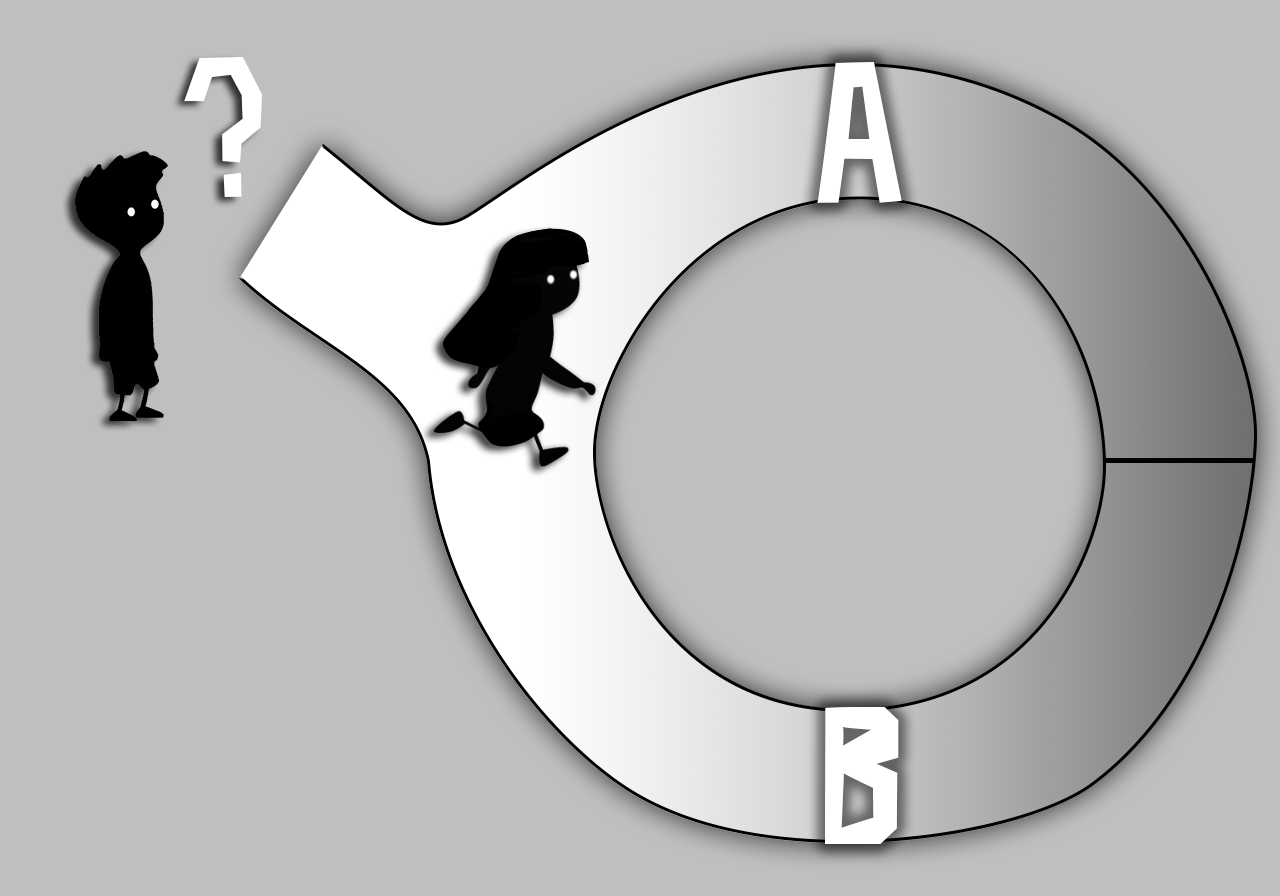
\includegraphics[width=1.\linewidth]{gfx/graficoJL_ZKP_1}\\La cueva \citep{ZKPcave:fig}. Peggy entra por A o B al azar. Víctor espera fuera.}
Peggy y Víctor quedan en la entrada de la cueva con unos \textit{walkie-talkies}, de modo que Víctor esperará fuera y Peggy entrará a la cueva y tomará uno de los pasillos, que llamaremos A y B, sin decirle cuál a Víctor.

%\begin{figure}[bth]
%	\begin{center}
%		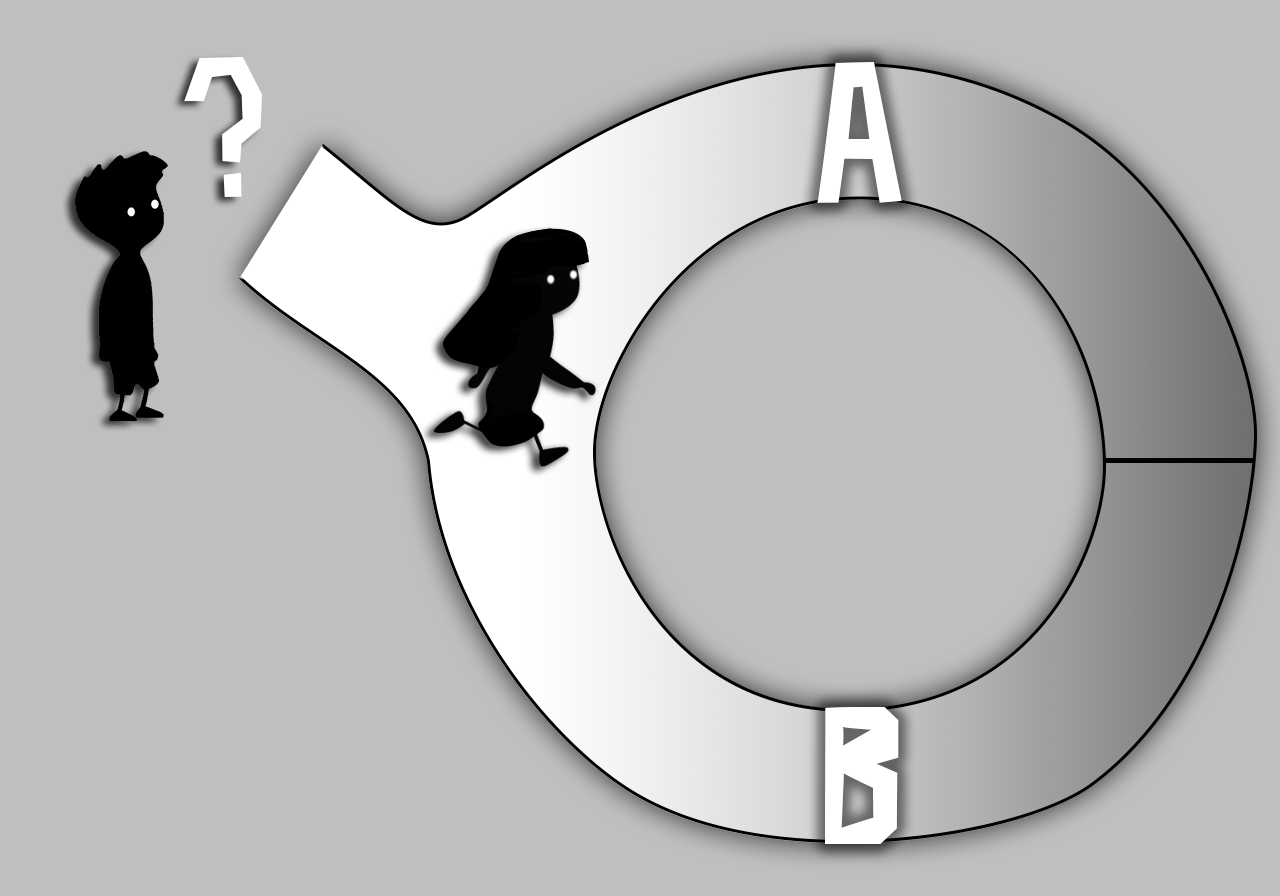
\includegraphics[width=.45\linewidth]{gfx/graficoJL_ZKP_1}
%	\end{center}
%	\caption{La cueva \citep{ZKPcave:fig}. Peggy entra por A o B al azar, Víctor espera fuera.}
%	\label{fig:ZKPcave1}
%\end{figure}

Al llegar a la puerta, avisa a Víctor para que entre a la cueva y espere en la bifurcación, donde \textbf{V}íctor, para intentar \textbf{v}erificar que Peggy conoce la clave, le indicará por qué pasillo quiere que vuelva, el A o el B.


%\begin{figure}[bth]
%	\begin{center}
%		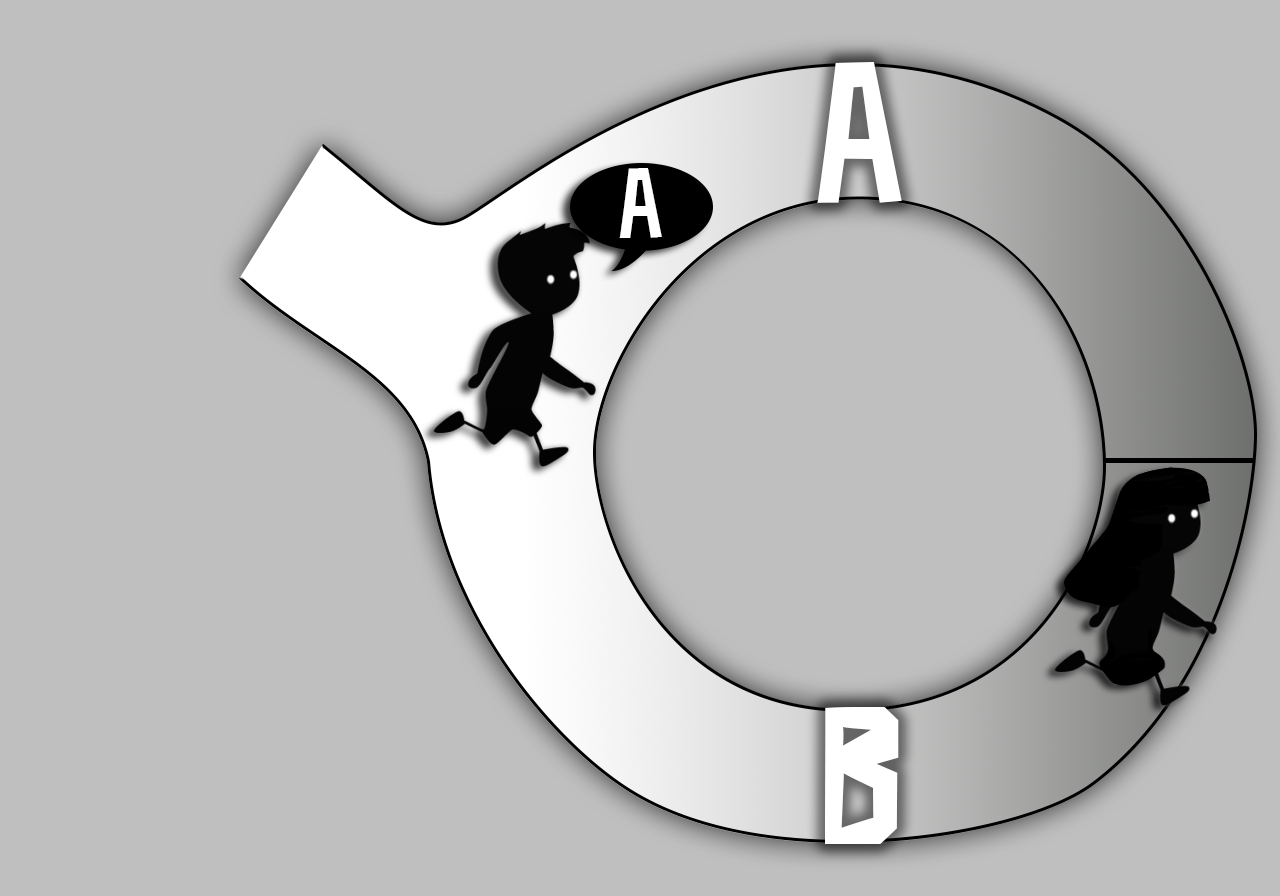
\includegraphics[width=.45\linewidth]{gfx/graficoJL_ZKP_2}
%	\end{center}
%	\caption{La cueva. Víctor elige al azar por dónde quiere que regrese Peggy.}
%	\label{fig:ZKPcave2}
%\end{figure}

Si Peggy realmente conoce la clave, podrá volver a la bifurcación por el pasillo solicitado, abriendo, si es preciso, la puerta.\marginpar{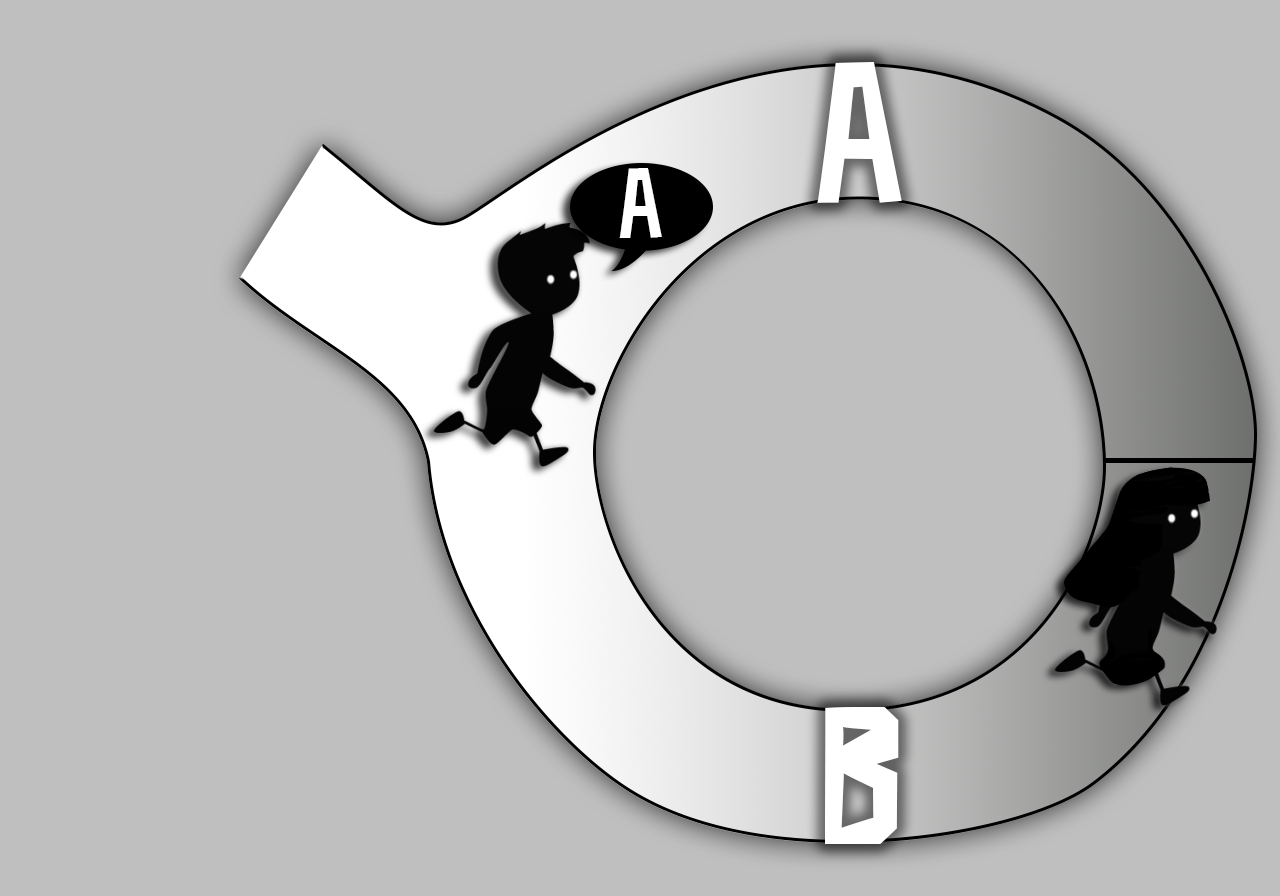
\includegraphics[width=1.\linewidth]{gfx/graficoJL_ZKP_2}\\La cueva. Víctor elige al azar por dónde quiere que regrese Peggy.}
En caso de que no conociera la clave, al entrar tenía una probabilidad del $50\%$ de adivinar qué pasillo pediría Víctor.


%\begin{figure}[bth]
%	\begin{center}
%		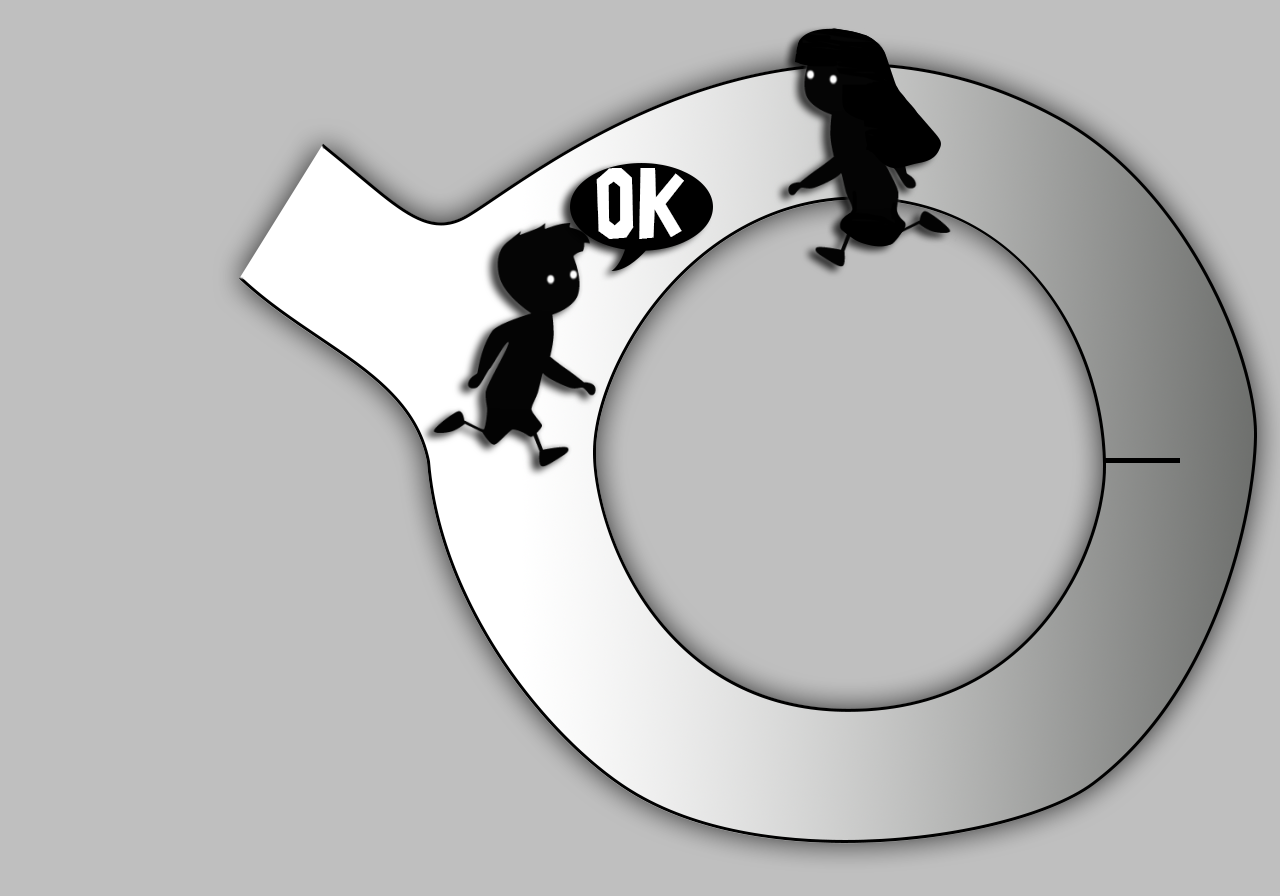
\includegraphics[width=.45\linewidth]{gfx/graficoJL_ZKP_3}
%	\end{center}
%	\caption{La cueva. Peggy vuelve por el camino pedido.}
%	\label{fig:ZKPcave3}
%\end{figure}

Víctor no se queda contento con una sola prueba, así que la repiten hasta que se convence. Si lo repitieran, por ejemplo, 20 veces, Peggy tendría solo una probabilidad de $2^{-20}$, prácticamente nula, de acertar todas las veces y engañar a Víctor.
\marginpar{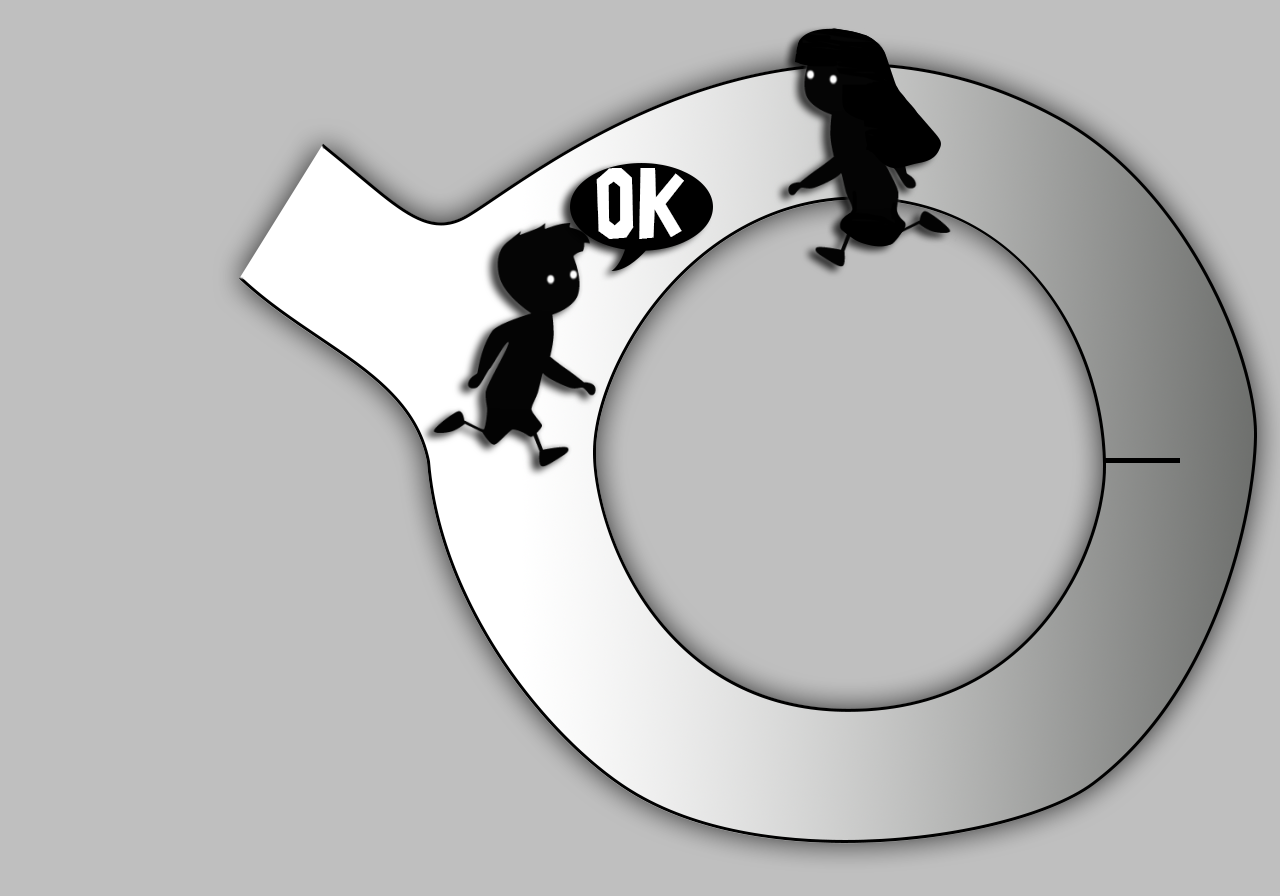
\includegraphics[width=1.\linewidth]{gfx/graficoJL_ZKP_3}\\La cueva. Peggy vuelve por el camino pedido.}


\textbf{E}va, curiosa de qué hacían Víctor y Peggy en la cueva, \textbf{e}spía a Víctor durante todo el proceso. Eva no sabe si Peggy y Víctor han acordado previamente qué pasillo pedir por el \textit{walkie-talkie}, y sólo Víctor está seguro de que los estaba eligiendo al azar, por eso, Eva no puede estar segura de si Peggy conoce la clave secreta, o bien estaban \textbf{s}imulando todo para engañarla por cotilla.

\hfil

\section{Sistema de Prueba Interactivo}

Un \textit{sistema de prueba interactivo} es un concepto de la teoría computacional que modela el intercambio de un número finito de mensajes entre dos partes, el probador P y el verificador V, con el objetivo de que P demuestre a V que una instancia de un problema de decisión es $Verdadera$. V tiene una capacidad de cómputo limitada, a lo sumo un algoritmo probabilístico de tiempo de cómputo polinomial. P es computacionalmente todopoderoso. Al final del intercambio de mensajes, o bien V acepta que la instancia es $Verdadera$, o bien la rechaza por ser $Falsa$.

\begin{definition}

	
	Se dice que un problema de decisión $Q$, no necesariamente en \textbf{NP},  tiene un \textit{sistema de prueba interactivo} si tiene un protocolo de interacción polinomialmente acotado en número de mensajes que cumple:
	
	\begin{itemize}
		\item \textit{Completitud} Para toda instancia $q$ $Verdadera$, del problema $Q$, V acepta $q$ como $Verdadera$. 
		\item  \textit{Robustez} Para cada instancia $q$ $Falsa$, ningún P, incluso si no sigue el protocolo, puede convencer a V de que $q$ es $Verdadera$, excepto con una pequeña probabilidad.
	\end{itemize}

\end{definition}

En resumen, si la instancia del problema $Q$ que P quiere demostrar es $Verdadera$, el protocolo siempre funciona, no hay falsos negativos, pero si la instancia es $Falsa$, hay una pequeña probabilidad de que $V$ la acepte como $Verdadera$, pueden haber falsos positivos una probabilidad casi despreciable.

Un P o un V que no siguen el protocolo e intentan romper estas propiedades, los llamaremos un P o V \textit{tramposos}.


\begin{definition}
	Denominamos clase de problemas \textbf{IP} (Interactivos en tiempo Polinomial) al conjunto de problemas de decisión para los que existe un sistema de prueba interactivo.
\end{definition}

\begin{proposition}
	\textbf{NP} $\subset$ \textbf{IP}.
\end{proposition}

\begin{proof}
	Sea $Q$ un problema \textbf{NP}. Definimos el siguiente protocolo:

	\begin{enumerate}
		\item  P resuelve la instancia del problema gracias a su capacidad de cómputo ilimitada y genera el certificado para V, que existe para cualquier instancia $Verdadera$ por $Q\in$ \textbf{NP}.
		\item  V recibe y puede verificar el certificado en tiempo polinomial. Si es válido, V acepta como $Verdadera$ la instancia. Si no, rechaza y devuelve que es $Falsa$.
	\end{enumerate}

	El protocolo es completo y robusto, con probabilidad nula de falso positivo, pues si la instancia es $Falsa$, ningún P, honesto o tramposo, puede generar un certificado que no existe.

\end{proof}


\hfil

\paragraph{Prueba Interactiva para el Problema QR}

\hfil

\hfil

Vamos a ver una prueba interactiva para demostrar que un entero $x$ con Símbolo de Jacobi 1 respecto a $n$, $x \in \mathbb{Z}^Q_n$, es un residuo cuadrático, $x \in \mathbb{Z}^{Q+}_n$.

\hfil

\begin{tabular}{|ll}
	\textit{Nombre:} & Problema QR. \\
	\textit{Parámetros:} & Un entero $N$ compuesto, y el entero $x\in \mathbb{Z}^Q_N$. \\
	\textit{Pregunta:} & ¿Es $x$ un residuo cuadrático, $x \in \mathbb{Z}^{Q+}_N$? \\
\end{tabular}
\\

\hfil

Una instancia $Verdadera$ del problema es un $x$ residuo cuadrático módulo $N$. Una prueba interactiva para demostrar que $x$ es residuo cuadrático es la siguiente:

\hfil

\rule{\textwidth}{1pt}
\begin{algorithm}[Prueba interactiva para QR]
	
	\hfil
	
	\textit{Datos comunes}: Una instancia ($x$, $N$) del Problema QR. $n$ es el tamaño de la instancia.
	
	\textit{Protocolo}: Sea $t(n)$ un polinomio en $n$. P y V repiten $t(n)$ veces los siguientes pasos.
	
	\begin{enumerate}
		
		\item P $\rightarrow$ V :\quad $u \in_R \mathbb{Z}^{Q+}_N$ \quad (P elige aleatoriamente $u$ en $\mathbb{Z}^{Q+}_N$).
		
		\item V $\rightarrow$ P :\quad $b \in_R \{0,\,1\}$.
		
		\item P $\rightarrow$ V :\; $w$,\; una raíz cuadrada módulo $N$ aleatoria, de $x$ si $b=0$, o bien de $x\cdot u$ si $b=1$.
		
		\item V comprueba si:
		\[
			w^2 \overset{?}{\equiv}
			\begin{cases}
				u\, mod\, N, & si\ b = 0\\
				xu\, mod\, N, & si\ b = 1.\\
			\end{cases}
		\]
		
		Si la comparación falla, V termina en rechazo, la instancia es $Falsa$. En caso contrario, vuelve al paso 1.
		
		
	\end{enumerate}

	Tras $t(n)$ rondas, V termina y acepta la instancia como $Verdadera$, $x$ es un residuo cuadrático módulo $N$.
	
	\label{QRinteractive:alg}
\end{algorithm}
\rule{\textwidth}{1pt}

\hfil


\begin{theorem}
	El problema QR tiene un sistema de prueba interactiva.
\end{theorem}

\begin{proof}
	
	El protocolo se ejecuta $t(n)$ veces, un número de iteraciones polinomialmente asociado al tamaño $n$ de la entrada, por lo que hay un número finito de mensajes que V, computacionalmente limitado, puede llevar a cabo. 
	
	\hfil 
	
	Queda ver que el protocolo anterior es completo y robusto.
	
	La prueba es \textit{completa}, pues para cualquier instancia $Verdadera$ de QR, $x \in \mathbb{Z}^{Q+}_N$, V acepta la prueba de P. En cada iteración, como P es computacionalmente todopoderoso, puede calcular $w$, una raíz cuadrada módulo $N$ de $x$ o $xu$, según el valor de $b$, ambos en $\mathbb{Z}^{Q+}_N$.
	
	Para una instancia $Falsa$, $x \in \mathbb{Z}^{Q-}_N$, cuando V envíe $b=1$, si P sigue el protocolo $u$ será un residuo cuadrático, pero $x\cdot u$ es un no-residuo cuadrático módulo $N$, por lo que no podrá calcular $w$ por mucho poder computacional ilimitado que tenga. Un P tramposo podría intentar engañar a V en el caso $b = 1$ eligiendo $u$ tal que $xu$ es un residuo cuadrático, pero entonces $u$ es un no-residuo cuadrático y fallaría la prueba si $b=0$.
	
	Una vez P se compromete con un $u$, residuo cuadrático o no, la probabilidad de que V lo rechace en esa iteración es $1\/2$, según elija $b=0$ ó $1$. Como el protocolo se ejecuta $t(n)$ veces, la probabilidad de que un P tramposo pueda engañara V en todos es de $2^{-t(n)}$. Vemos entonces que el protocolo cumple la propiedad de \textit{robustez}.
\end{proof}


% TODO: para la presentación, si preguntan por qué t(n) depende del tamaño de la entrada, preparar ejemplo de Z_5 o Z_15 mejor, por 15=3*5 los primos impares, indicar que hay 7 residuos cuadráticos y 7 no-residuos, que la cantidad de u's distintos que puede tomar aleatoriamente de entre los rq y los no-rq para intentar engañarlo es mínima, y en pocas iteraciones pueden haber probado todas las combinaciones, y seguir el protocolo es repetir valores ya contrastados, y comparando con primos de 2048 bits, se pueden pedir más iteraciones.


\section{Pruebas de conocimiento cero}

% Introducción: De manera informal,....
% Definiciones: Prueba de conocimiento (como subconjunto de pruebas de problemas de decisión?), Ensemble, View, Simulator

%TODO: ahora que se habla más de un secreto, que es lo que queremos mantener privado en P, demostrar de la robustez, que si un cheating P no conoce el secreto, pero pasa la prueba, tiene un conocimiento equivalente al secreto. Dem por tema de la probabilidad.

\subsection{Pruebas de conocimiento cero perfectas}

\subsection{Pruebas de conocimiento cero estadísticas}

\subsection{Pruebas de conocimiento cero computacionales}


\section{Protocolos de identificación basados en ZKP}
% Puede que para el siguiente capítulo
% Fiat-Shamir, FFS, GQ, Schnorr

